\begin{appendices}

%
% The first appendix must be "Self-appraisal".
%
\chapter{Self-appraisal}
\section{Critical self-evaluation}
Overall, I am very pleased with this project. From the beginning this project was quite ambitious; however, I was able to achieve the goals initially set out at the start of the project.
\\Although this project was successful, this doesn't by any means imply that it was easy. Having no experience with RL nor Planning meant that I had a lot to learn in a short amount of time. It was sufficient for me to understand Planning at a high-level, however I had to \textit{really} understand RL. Sutton and Barto's "Reinforcement Learning: An Introduction" \cite{Sutton1998} was a constant companion to me, alongside many other resources and research papers. Over the course of this project, I became obsessed with RL and understanding how and why it works; thus, I developed a strong intuition for RL which was foundational in the success of this project.
\\My conversations with my supervisors were really insightful, and I often found myself fascinated within our conversations. However, I found that often I struggled to articulate my ideas, which led to us not being on the same page; this is definitely something that I need to improve upon. Similarly, I had difficulties articulating my ideas on paper, therefore writing the report was very time consuming, although I got there in the end.
\\ Coming up with ideas is a challenging and interesting process. The overall idea of the framework and use of Meta Actions was there from the beginning. However, encapsulating that idea involves coming up with various other ideas. I am most pleased with the idea that I came up with for the modified version of Value Iteration; it actually makes sense as a solution, due to the evaluative nature of VI.
\\ In terms of implementing my ideas, I did not struggle, for the most part. Although when I did run into problems, which are inevitable in software development, it could be quite difficult to discover exactly where things were going wrong. Perhaps, if I had more logging-style functionality, it would be easier to trace back unexpected behaviour, and solve issues more quickly. However, I was a bit stubborn and didn't do that.
\\ My project planning and management was definitely my weakest point. I often found myself lacking direction and contemplating what I was actually supposed to be doing. If I planned more thoroughly in the beginning and actually stuck to it, I could have been a lot more successful, and perhaps had more time for further research.
\\ I often found myself going back and improving my ideas. On the one hand this was good, because I was able to identify weaknesses in my approaches and improve them. On the other hand, this was to my detriment. I kept going back and changing things, when I should've been spending more times evaluating my ideas; even when told by my supervisors that I should be doing this, I couldn't help myself.
\\In conclusion, this project was a success. However, it could have been more successful if I planned better and set strict deadlines for development.
% This meant that I had to undertake lots of research to bring myself up-to-speed. Most of this research took place on the RL side of things, with 



% \\Before this project, I had no experience with Reinforcement Learning nor Planning, and lacked experience in developing novel algorithms more generally. 




% \begin{itemize}
%     \item Success overall; what was achieved.
%     \item Shortcomings, how they could have been avoided
    
% \end{itemize}

\section{Personal reflection and lessons learned}
On a personal level, I am very pleased with my growth throughout this project. I was able to go from knowing nothing about RL, to being quite knowledgeable about it. Furthermore, I realised that I want to pursue a career where I can continue research into RL.
\\The biggest lesson that I learned was the importance of project planning. I believe my project could've been much more successful if I maintained a clearer idea of the project formulated through a plan. In future projects, I am certainly going to put more time and effort into planning.
\\Another big lesson that I learned was that benchmarking should be a continual part of research, not something that should be done at the end. Furthermore, standard benchmarks should be considered rather than developing benchmarks on our own. I learned this the hard way, I introduced my own "biases" when developing my own benchmarks which looking back now having done \textit{proper} benchmarking, led to misconceptions about performance.
\\Research never ends. This lesson was a hard one to learn. As I mentioned in my critical self-evaluation, I often found myself returning to my algorithms and making improvements, due to my perfectionist nature. However, one needs to understand that research is, potentially, infinite; there will always be some improvement to be made, but they don't all have to be made in the current piece of work, they can be left for future research.

\section{Legal, social, ethical and professional issues}
The legal, social, ethical and professional issues mostly relate to the potential use cases of this project, rather than the project itself. This project did not produce a \textit{complete} framework that can be deployed straight into the real-world, however in this section we will discuss under the assumption that this is a possibility.
\subsection{Legal issues}
In general, the major legal concern relating to AI is liability; who is to blame for a mistake made by an AI? If our framework was used by some company, and it resulted in an accident where someone got hurt, who would be to blame? Would it be us, who developed the framework, the engineer who implemented and trained it, or the company itself? Another legal concern pertains to data. If a company used data (potentially belonging to individuals), then they should have the legal authority to use such data.
\\Within our project, use of external libraries and figures were referenced, where appropriate, and used with their associated licenses in mind. This ensured use of external libraries and figures was done legally.
% Data used by a potential company during training shou
% % Would it be us, who developed the framework, the engineer who trained it for their companies use case, the company itself? More legal issues may arise during training, specifically if data is being supplemented; the company training must have the legal authority to use such data.

% The major concern, of a legal nature, with Artificial Intelligence (AI) 
% The use of Reinforcement Learning (RL) also raises important legal issues that need to be addressed. One major concern is liability: who is responsible when an RL agent causes harm? This is particularly challenging when the agent's behavior is unpredictable or beyond human understanding. Additionally, there may be legal questions around ownership of the data used to train RL systems, as well as issues related to privacy and data protection. To address these legal issues, it is essential to establish clear legal frameworks and standards for the development and use of RL systems. This can include regulations around the use of RL in certain industries or applications, as well as legal requirements for transparency and accountability in the development and deployment of RL agents. Additionally, it may be necessary to establish liability frameworks that take into account the unique characteristics of RL, such as the complexity of the decision-making process and the potential for unpredictable behavior. By addressing these legal issues, we can ensure that the development and use of RL is consistent with our legal principles and protections, and that the benefits of RL are realized while minimizing the risks to individuals and society.
\subsection{Social issues}
A commonly discussed issue in the context of AI is that it will "replace humans", leading to unemployment. However, this can be omitted by offering retraining to those individuals who have had their jobs automated in order to ensure that they remain skilled and employable.
% The use of Reinforcement Learning (RL) can also raise societal issues that need to be considered. One of the primary concerns is the potential impact of RL on employment and income inequality. As RL algorithms are developed to automate tasks that were previously done by humans, there is a risk that large numbers of workers could lose their jobs, leading to increased income inequality. Additionally, there is a possibility that RL systems could be used to unfairly manipulate markets or influence political decisions. To mitigate these societal issues, it is important to consider the broader impact of RL on society and to ensure that its benefits are distributed fairly. This can include investing in retraining programs for workers whose jobs may become automated, regulating the use of RL systems in sensitive areas such as finance and politics, and promoting the development of RL applications that contribute to the public good. By taking a proactive approach to addressing these societal issues, we can ensure that the development and use of RL aligns with our shared values and aspirations for a just and equitable society.
% The primary social issue pertaining AI in general is that of causing unemployment, through automating menial tasks previously done by humans. However, this could be 
\subsection{Ethical issues}
The main ethical concerns with AI are bias and fairness. In the context of RL, bias could be introduced during learning. Bias could be avoided and fairness guaranteed by not only optimising to achieve the maximum cumulative reward, but also to maximise some fairness objective/minimise some bias objective. However, humans are normally responsible for constructing the reward function of an environment, which can ultimately influence the behaviour of any agents that learn through it.


% Bias can be introduced into an RL system during learning, however this could be omitted by adding additional objectives, alongside maximising cumulative reward, such as maximising some fairness objective.
% Furthermore, since a human is responsible for constructing the reward function, they can ultimately influence the behaviour of an RL system.
\subsection{Professional issues}
This project was carried out in-line with the British Computing Society Code of Conduct
\cite{bcs}. Most notably, we ensured that we did not misrepresent our proposed methods by presenting false results. Furthermore, we ensured that any external work was attributed correctly, through thorough referencing and providing links to external material in the appendices.

%
% Any other appendices you wish to use should come after "Self-appraisal". You can have as many appendices as you like.
%
\chapter{External Material}
https://github.com/ibrahim-elshar/gym-windy-gridworlds

\chapter{Domains}

\begin{figure}[H]
    \centering
    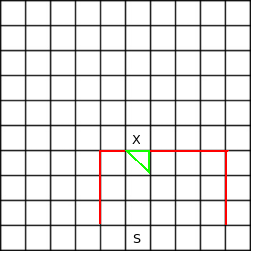
\includegraphics[max size={250}{250}]{report/assets/envs/gridworld.png}
    \caption{Gridworld Domain}
    \label{fig:grid_domain}
\end{figure}

\begin{figure}[H]
    \centering
    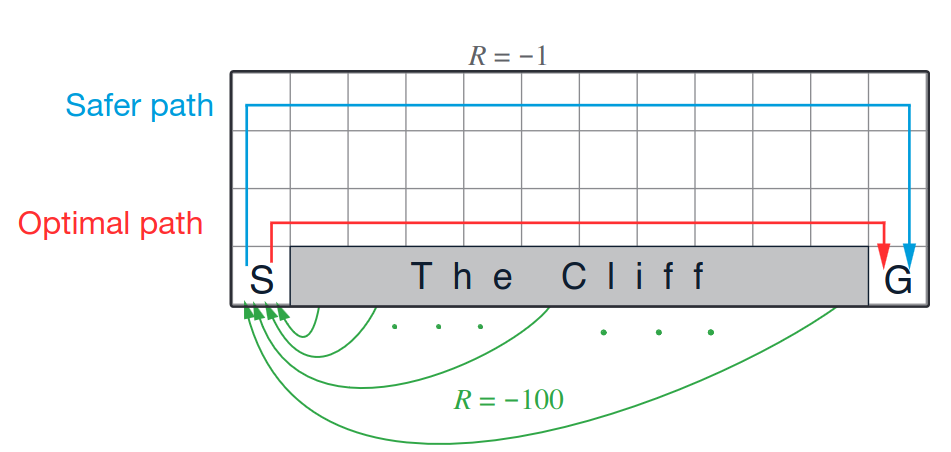
\includegraphics[max size={250}{250}]{report/assets/envs/cliff-walking.png}
    \caption{Cliff-Walking Domain \cite{Sutton1998}}
    \label{fig:cliff_walking}
\end{figure}

\begin{figure}[H]
    \centering
    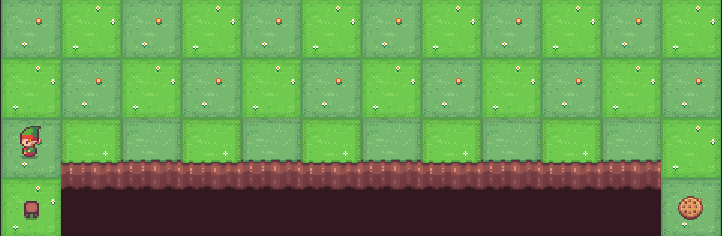
\includegraphics[max size={250}{250}]{report/assets/envs/cliff_walking_domain.png}
    \caption{Cliff-Walking Domain \cite{1606.01540}}
    \label{fig:cliff_walking_openai}
\end{figure}

\begin{figure}[H]
    \centering
    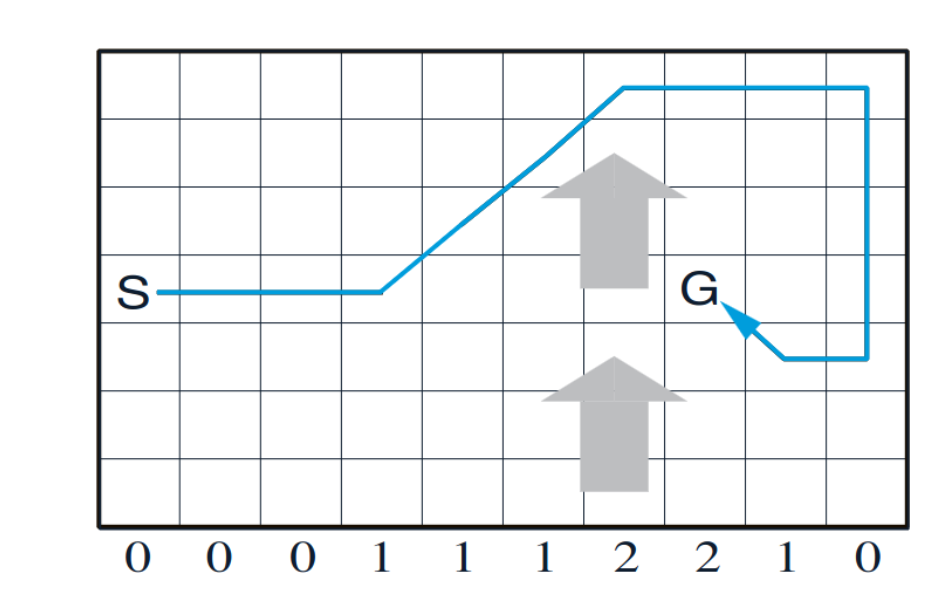
\includegraphics[max size={250}{250}]{report/assets/envs/windy.png}
    \caption{Windy Gridworld Domain \cite{Sutton1998}}
    \label{fig:windy_gridworld}
\end{figure}

\begin{figure}[H]
    \centering
    
\includegraphics[max size={250}{250}]{report/assets/envs/frozen-lake.png}
    \caption{Frozen Lake Domain \cite{1606.01540}}
    \label{fig:frozen_lake}
\end{figure}


%
% Other appendices can be added here following the same pattern as above.
%



% \chapter{Further Studies}
% \section{Ablation Studies}


% \section{Generalisation}

\end{appendices}
